\chapter{WF-167 Roadmap Milestone Authority}\label{record-249}

\noindent{\footnotesize\color{BookMuted}\path{docs/design/WF-167-roadmap-milestone-authority.md}\par}\smallskip

Legend: \href{https://github.com/flyingrobots/bijou/blob/1853ad902f6bf219326409e7f743a5a1d6517dbc/docs/legends/WF-workflow-and-delivery.md}{WF --- Workflow and Delivery}

Tracker: \href{https://github.com/flyingrobots/bijou/issues/514}{\#514}

\section{Sponsor Human}\label{record-249-sponsor-human}

James Ross.

\section{Sponsor Agent}\label{record-249-sponsor-agent}

Codex.

\section{Decision Summary}\label{record-249-decision-summary}

Restore one explainable release model across GitHub milestones, \href{https://github.com/flyingrobots/bijou/blob/5b10cb89165b76673ffc60da59d7de5a531e55e9/docs/ROADMAP.md}{\texttt{R\allowbreak{}O\allowbreak{}A\allowbreak{}D\allowbreak{}M\allowbreak{}A\allowbreak{}P\allowbreak{}.\allowbreak{}m\allowbreak{}d}}, and \href{https://github.com/flyingrobots/bijou/blob/5b10cb89165b76673ffc60da59d7de5a531e55e9/docs/BEARING.md}{\texttt{B\allowbreak{}E\allowbreak{}A\allowbreak{}R\allowbreak{}I\allowbreak{}N\allowbreak{}G\allowbreak{}.\allowbreak{}m\allowbreak{}d}}.

Milestones own release horizons. Labels own work posture. Goalpost issues own dependency ordering inside a horizon. Documentation mirrors those authorities; it does not create a competing queue.

The current \texttt{v\allowbreak{}8\allowbreak{}.\allowbreak{}0\allowbreak{}.\allowbreak{}0} milestone mixes a landed Runtime Graph and Scene IR contract, an active dependency-security blocker, an additive open Theme Lab pull request, and twenty-one unfinished perceptual-colour and product-surface issues. The unfinished colour campaign includes changes explicitly identified as semver-major. It belongs before the next major release, \texttt{v\allowbreak{}9\allowbreak{}.\allowbreak{}0\allowbreak{}.\allowbreak{}0}, rather than becoming a second product contract inside V8.

This cycle therefore:

\begin{enumerate}
\def\labelenumi{\arabic{enumi}.}
\tightlist
\item
  returns \texttt{v\allowbreak{}8\allowbreak{}.\allowbreak{}0\allowbreak{}.\allowbreak{}0} to Runtime Graph release closeout and dependency security;
\item
  preserves \texttt{v\allowbreak{}8\allowbreak{}.\allowbreak{}1\allowbreak{}.\allowbreak{}0} as replay, capture, debugger, graph, and render evidence;
\item
  preserves \texttt{v\allowbreak{}8\allowbreak{}.\allowbreak{}2\allowbreak{}.\allowbreak{}0} as quality automation and reliability hardening;
\item
  makes \texttt{v\allowbreak{}9\allowbreak{}.\allowbreak{}0\allowbreak{}.\allowbreak{}0} the Product Workbench \textbf{and Sapphire Design Language} major, including interaction recipes and the State Atlas;
\item
  keeps \texttt{v\allowbreak{}1\allowbreak{}0\allowbreak{}.\allowbreak{}0\allowbreak{}.\allowbreak{}0} for renderer and host integration, including the Geordi native-GPU cell host;
\item
  removes stale title and label residue created by earlier Beyond-to-version promotion;
\item
  assigns every open pull request to its evidenced release horizon.
\end{enumerate}

No issue closes in this cycle. No implementation priority is inferred merely from a milestone move.

\section{Hill}\label{record-249-hill}

A maintainer or agent can answer all of these from the live tracker and receive the same answer from the repository documentation:

\begin{itemize}
\tightlist
\item
  What blocks V8?
\item
  Which work is evidence follow-through rather than release closeout?
\item
  Which visual changes belong to the next semver-major boundary?
\item
  Which ideas are committed, imminent, debt, or optional?
\item
  Which open pull requests participate in each release horizon?
\item
  What must be reconciled before an overlapping pull request can merge?
\end{itemize}

The answer must not require reading historical comments, inferring semantics from an issue number, or treating a \texttt{l\allowbreak{}a\allowbreak{}n\allowbreak{}e\allowbreak{}:\allowbreak{}c\allowbreak{}o\allowbreak{}o\allowbreak{}l\allowbreak{}-\allowbreak{}i\allowbreak{}d\allowbreak{}e\allowbreak{}a\allowbreak{}s} label as a release commitment.

\section{Current Truth}\label{record-249-current-truth}

The pre-cycle snapshot was taken from GitHub on 2026-08-09 against \texttt{o\allowbreak{}r\allowbreak{}i\allowbreak{}g\allowbreak{}i\allowbreak{}n\allowbreak{}/\allowbreak{}m\allowbreak{}a\allowbreak{}i\allowbreak{}n} at \texttt{4\allowbreak{}4\allowbreak{}1\allowbreak{}2\allowbreak{}e\allowbreak{}c\allowbreak{}6\allowbreak{}d\allowbreak{}b\allowbreak{}c\allowbreak{}e\allowbreak{}9\allowbreak{}4\allowbreak{}7\allowbreak{}8\allowbreak{}8\allowbreak{}7\allowbreak{}e\allowbreak{}d\allowbreak{}6\allowbreak{}e\allowbreak{}a\allowbreak{}2\allowbreak{}7\allowbreak{}4\allowbreak{}0\allowbreak{}e\allowbreak{}c\allowbreak{}b\allowbreak{}a\allowbreak{}d\allowbreak{}0\allowbreak{}a\allowbreak{}6\allowbreak{}6\allowbreak{}d\allowbreak{}1\allowbreak{}2\allowbreak{}2\allowbreak{}e}.

\subsection{Milestone Items Before This Cycle}\label{record-249-milestone-items-before-this-cycle}

GitHub milestone totals count issues and pull requests:

\begin{center}
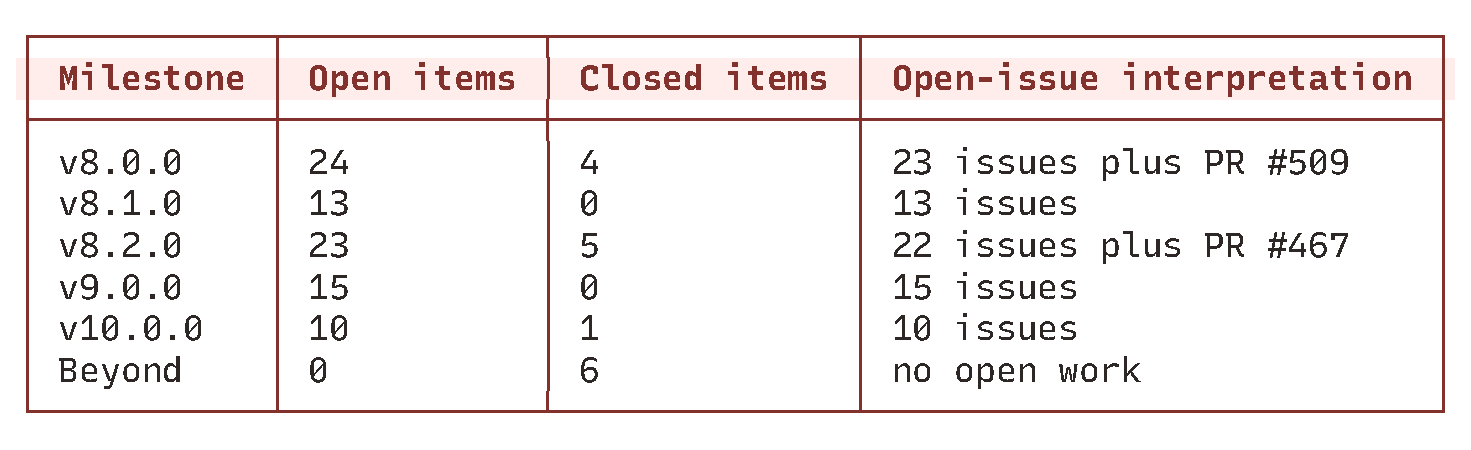
\includegraphics[width=\linewidth]{figures/tables/table-062-g1-1.pdf}
\par\smallskip{\scriptsize\color{BookMuted}Rows 1–6. Actual Bijou table component.}
\end{center}


Two additional open pull requests were unmilestoned:

\begin{itemize}
\tightlist
\item
  V8 dependency-security PR \href{https://github.com/flyingrobots/bijou/pull/492}{\#492};
\item
  V10 Geordi native-GPU design PR \href{https://github.com/flyingrobots/bijou/pull/511}{\#511}.
\end{itemize}

The audit cohort therefore contained \texttt{8\allowbreak{}3} open issues and \texttt{4} open pull requests. Opening governance issue \#514 increases the live issue total to \texttt{8\allowbreak{}4}; opening governance PR \#515 increases the open pull request total to \texttt{5}. Both live in the \texttt{v\allowbreak{}8\allowbreak{}.\allowbreak{}2\allowbreak{}.\allowbreak{}0} milestone during the cycle.

\subsection{V8 Scope Drift}\label{record-249-v8-scope-drift}

The landed V8 source-side contract is carried by:

\begin{itemize}
\tightlist
\item
  closed parent tracker \href{https://github.com/flyingrobots/bijou/issues/302}{\#302};
\item
  closed goalpost \href{https://github.com/flyingrobots/bijou/issues/457}{\#457};
\item
  landed VISOR artifact bundle \href{https://github.com/flyingrobots/bijou/issues/458}{\#458};
\item
  landed packed-cell adapter \href{https://github.com/flyingrobots/bijou/issues/459}{\#459}.
\end{itemize}

The active release prerequisite is dependency-security issue \href{https://github.com/flyingrobots/bijou/issues/482}{\#482}. Pull requests \#492 and \#509 overlap on that remediation and must be deduplicated before either is selected for merge.

Issue \#501 was subsequently retargeted from V9 into V8 with its foundation, correctness, Theme Lab, title-screen, and surface issues. That decision made the V8 release gate depend on work whose own tracker identifies three semver-major output changes:

\begin{itemize}
\tightlist
\item
  \#496 changes theme decision-rule results;
\item
  \#497 changes every first-party theme colour;
\item
  \#499 changes ANSI-256 rendered output.
\end{itemize}

Those changes can land honestly before \texttt{v\allowbreak{}9\allowbreak{}.\allowbreak{}0\allowbreak{}.\allowbreak{}0}. They need not hold the already landed V8 product contract open.

\subsection{Tracker Hygiene Drift}\label{record-249-tracker-hygiene-drift}

The live tracker also contains mechanically identifiable residue:

\begin{itemize}
\tightlist
\item
  issues promoted out of \texttt{B\allowbreak{}e\allowbreak{}y\allowbreak{}o\allowbreak{}n\allowbreak{}d} retain \texttt{[\allowbreak{}B\allowbreak{}e\allowbreak{}y\allowbreak{}o\allowbreak{}n\allowbreak{}d\allowbreak{}]} in their titles;
\item
  \#204 carries both \texttt{l\allowbreak{}a\allowbreak{}n\allowbreak{}e\allowbreak{}:\allowbreak{}i\allowbreak{}n\allowbreak{}b\allowbreak{}o\allowbreak{}x} and \texttt{l\allowbreak{}a\allowbreak{}n\allowbreak{}e\allowbreak{}:\allowbreak{}c\allowbreak{}o\allowbreak{}o\allowbreak{}l\allowbreak{}-\allowbreak{}i\allowbreak{}d\allowbreak{}e\allowbreak{}a\allowbreak{}s};
\item
  \#214, \#217, and \#218 carry both current \texttt{l\allowbreak{}a\allowbreak{}n\allowbreak{}e\allowbreak{}:\allowbreak{}c\allowbreak{}o\allowbreak{}o\allowbreak{}l\allowbreak{}-\allowbreak{}i\allowbreak{}d\allowbreak{}e\allowbreak{}a\allowbreak{}s} and legacy \texttt{l\allowbreak{}a\allowbreak{}n\allowbreak{}e\allowbreak{}:\allowbreak{}u\allowbreak{}p\allowbreak{}-\allowbreak{}n\allowbreak{}e\allowbreak{}x\allowbreak{}t};
\item
  \#219 remains \texttt{l\allowbreak{}a\allowbreak{}n\allowbreak{}e\allowbreak{}:\allowbreak{}i\allowbreak{}n\allowbreak{}b\allowbreak{}o\allowbreak{}x} despite an explicit V10 horizon;
\item
  \#348 remains \texttt{l\allowbreak{}a\allowbreak{}n\allowbreak{}e\allowbreak{}:\allowbreak{}a\allowbreak{}s\allowbreak{}a\allowbreak{}p} despite an explicit V10 horizon;
\item
  \#249 carries both \texttt{p\allowbreak{}r\allowbreak{}i\allowbreak{}o\allowbreak{}r\allowbreak{}i\allowbreak{}t\allowbreak{}y\allowbreak{}:\allowbreak{}m\allowbreak{}e\allowbreak{}d\allowbreak{}i\allowbreak{}u\allowbreak{}m} and \texttt{p\allowbreak{}r\allowbreak{}i\allowbreak{}o\allowbreak{}r\allowbreak{}i\allowbreak{}t\allowbreak{}y\allowbreak{}:\allowbreak{}l\allowbreak{}o\allowbreak{}w};
\item
  \#507 is \texttt{l\allowbreak{}a\allowbreak{}n\allowbreak{}e\allowbreak{}:\allowbreak{}b\allowbreak{}a\allowbreak{}d\allowbreak{}-\allowbreak{}c\allowbreak{}o\allowbreak{}d\allowbreak{}e} but lacks the repository's normal \texttt{B\allowbreak{}A\allowbreak{}D\allowbreak{} \allowbreak{}C\allowbreak{}O\allowbreak{}D\allowbreak{}E\allowbreak{}:} title signal;
\item
  milestone descriptions do not mention the recently added interaction-state, State Atlas, or native-GPU stories.
\end{itemize}

These are tracker defects, not implementation defects.

\section{Authority Model}\label{record-249-authority-model}

\subsection{Milestone: Release Destination}\label{record-249-milestone-release-destination}

A versioned milestone answers: \textbf{if this work lands, which release boundary owns it?}

A milestone does not mean every issue is committed or next. That posture comes from \texttt{l\allowbreak{}a\allowbreak{}n\allowbreak{}e\allowbreak{}:\allowbreak{}*}, \texttt{w\allowbreak{}o\allowbreak{}r\allowbreak{}k\allowbreak{}-\allowbreak{}i\allowbreak{}n\allowbreak{}-\allowbreak{}p\allowbreak{}r\allowbreak{}o\allowbreak{}g\allowbreak{}r\allowbreak{}e\allowbreak{}s\allowbreak{}s}, priority, design, and goalpost labels.

\subsection{Lane: Commitment And Intake Posture}\label{record-249-lane-commitment-and-intake-posture}

\begin{itemize}
\tightlist
\item
  \texttt{l\allowbreak{}a\allowbreak{}n\allowbreak{}e\allowbreak{}:\allowbreak{}i\allowbreak{}n\allowbreak{}b\allowbreak{}o\allowbreak{}x}: not yet shaped;
\item
  \texttt{l\allowbreak{}a\allowbreak{}n\allowbreak{}e\allowbreak{}:\allowbreak{}a\allowbreak{}s\allowbreak{}a\allowbreak{}p}: imminent pull;
\item
  \texttt{l\allowbreak{}a\allowbreak{}n\allowbreak{}e\allowbreak{}:\allowbreak{}b\allowbreak{}a\allowbreak{}d\allowbreak{}-\allowbreak{}c\allowbreak{}o\allowbreak{}d\allowbreak{}e}: known debt or structural risk;
\item
  \texttt{l\allowbreak{}a\allowbreak{}n\allowbreak{}e\allowbreak{}:\allowbreak{}c\allowbreak{}o\allowbreak{}o\allowbreak{}l\allowbreak{}-\allowbreak{}i\allowbreak{}d\allowbreak{}e\allowbreak{}a\allowbreak{}s}: optional or uncommitted exploration;
\item
  \texttt{l\allowbreak{}a\allowbreak{}n\allowbreak{}e\allowbreak{}:\allowbreak{}r\allowbreak{}e\allowbreak{}l\allowbreak{}e\allowbreak{}a\allowbreak{}s\allowbreak{}e}: committed release-boundary work.
\end{itemize}

An issue should carry one current lane. Historical \texttt{l\allowbreak{}a\allowbreak{}n\allowbreak{}e\allowbreak{}:\allowbreak{}u\allowbreak{}p\allowbreak{}-\allowbreak{}n\allowbreak{}e\allowbreak{}x\allowbreak{}t} residue does not coexist with the current lane model.

\subsection{Goalpost: Dependency And Outcome Authority}\label{record-249-goalpost-dependency-and-outcome-authority}

Goalpost issues such as \#501 own dependency ordering within a release horizon. Moving a goalpost and its children between release horizons does not reorder the children. It changes the release boundary that may claim them.

\subsection{Documentation: Human-Readable Mirror}\label{record-249-documentation-human-readable-mirror}

\texttt{R\allowbreak{}O\allowbreak{}A\allowbreak{}D\allowbreak{}M\allowbreak{}A\allowbreak{}P\allowbreak{}.\allowbreak{}m\allowbreak{}d} records release horizons, gates, and snapshot totals. \texttt{B\allowbreak{}E\allowbreak{}A\allowbreak{}R\allowbreak{}I\allowbreak{}N\allowbreak{}G\allowbreak{}.\allowbreak{}m\allowbreak{}d} records current execution gravity. Neither file overrides live GitHub state.

\section{Target Milestone Model}\label{record-249-target-milestone-model}

\subsection{\texorpdfstring{\texttt{v\allowbreak{}8\allowbreak{}.\allowbreak{}0\allowbreak{}.\allowbreak{}0}: Runtime Graph Release Closeout}{: Runtime Graph Release Closeout}}\label{record-249-v8.0.0-runtime-graph-release-closeout}

Outcome:

\begin{itemize}
\tightlist
\item
  Runtime Graph and Scene IR product contract is landed;
\item
  dependency advisories reach zero through one selected remediation path;
\item
  release preparation begins only after security truth is reproducible;
\item
  no unfinished colour-system campaign blocks the release.
\end{itemize}

Expected open items after triage:

\begin{itemize}
\tightlist
\item
  issue \#482;
\item
  PR \#492;
\item
  PR \#509.
\end{itemize}

The two PRs overlap. Their simultaneous presence records alternatives, not three independent release blockers.

\subsection{\texorpdfstring{\texttt{v\allowbreak{}8\allowbreak{}.\allowbreak{}1\allowbreak{}.\allowbreak{}0}: Replay, Capture, And Render Evidence}{: Replay, Capture, And Render Evidence}}\label{record-249-v8.1.0-replay-capture-and-render-evidence}

No issue migration is required. The milestone remains the post-contract proof horizon for replay, capture, debugger, graph, browser, terminal, and parity witnesses.

Expected open items after triage: \texttt{1\allowbreak{}3}.

\subsection{\texorpdfstring{\texttt{v\allowbreak{}8\allowbreak{}.\allowbreak{}2\allowbreak{}.\allowbreak{}0}: Quality Automation And Reliability}{: Quality Automation And Reliability}}\label{record-249-v8.2.0-quality-automation-and-reliability}

Add issue \#507 because startup key-conflict reporting is quality enforcement, not Runtime Graph release scope. Governance issue \#514 also lives here because tracker synchronization is an explicit V8.2 outcome.

Expected open items after triage: \texttt{2\allowbreak{}6}:

\begin{itemize}
\tightlist
\item
  \texttt{2\allowbreak{}4} open issues, including \#507 and \#514;
\item
  Dependabot PR \#467;
\item
  governance PR \#515.
\end{itemize}

\subsection{\texorpdfstring{\texttt{v\allowbreak{}9\allowbreak{}.\allowbreak{}0\allowbreak{}.\allowbreak{}0}: Product Workbench And Sapphire Design Language}{: Product Workbench And Sapphire Design Language}}\label{record-249-v9.0.0-product-workbench-and-sapphire-design-language}

Move the full unfinished campaign cohort from V8:

\begin{center}
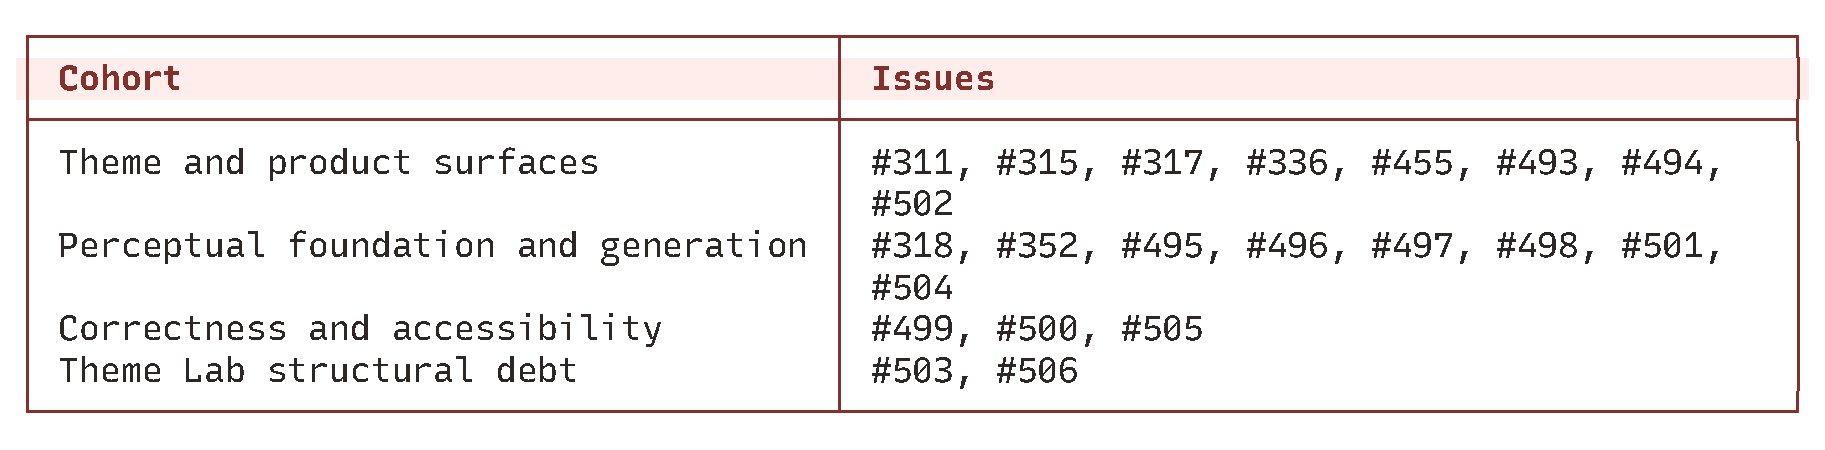
\includegraphics[width=\linewidth]{figures/tables/table-063-g1-1.pdf}
\par\smallskip{\scriptsize\color{BookMuted}Rows 1–4. Actual Bijou table component.}
\end{center}


The cohort contains \texttt{2\allowbreak{}1} issues. It joins the existing \texttt{1\allowbreak{}5} V9 issues, including interaction recipes \#512 and State Atlas \#513.

Expected open items after triage: \texttt{3\allowbreak{}6}.

The count is large because this milestone is an explicit future major horizon, not because all \texttt{l\allowbreak{}a\allowbreak{}n\allowbreak{}e\allowbreak{}:\allowbreak{}c\allowbreak{}o\allowbreak{}o\allowbreak{}l\allowbreak{}-\allowbreak{}i\allowbreak{}d\allowbreak{}e\allowbreak{}a\allowbreak{}s} work has become committed. \#501 and the existing Product Workbench stories provide the internal goalposts.

\subsection{\texorpdfstring{\texttt{v\allowbreak{}1\allowbreak{}0\allowbreak{}.\allowbreak{}0\allowbreak{}.\allowbreak{}0}: Renderer And Host Systems Integration}{: Renderer And Host Systems Integration}}\label{record-249-v10.0.0-renderer-and-host-systems-integration}

Keep the existing ten issues. Assign PR \#511 to the milestone and update the description to name the Geordi native-GPU cell-host boundary.

Expected open items after triage: \texttt{1\allowbreak{}1}.

\subsection{\texorpdfstring{\texttt{B\allowbreak{}e\allowbreak{}y\allowbreak{}o\allowbreak{}n\allowbreak{}d}: Deliberate Incubation}{: Deliberate Incubation}}\label{record-249-beyond-deliberate-incubation}

No issue moves into \texttt{B\allowbreak{}e\allowbreak{}y\allowbreak{}o\allowbreak{}n\allowbreak{}d} during this cycle. Explicit release destinations remain useful. The stale title prefix is removed from issues that already have a versioned destination.

\section{Issue Title And Label Normalization}\label{record-249-issue-title-and-label-normalization}

\subsection{\texorpdfstring{Remove Stale \texttt{[\allowbreak{}B\allowbreak{}e\allowbreak{}y\allowbreak{}o\allowbreak{}n\allowbreak{}d\allowbreak{}]} Prefix}{Remove Stale  Prefix}}\label{record-249-remove-stale-beyond-prefix}

Rename these open issues without changing their substantive titles:

\begin{itemize}
\tightlist
\item
  \#202 through \#219 where the current title begins \texttt{[\allowbreak{}B\allowbreak{}e\allowbreak{}y\allowbreak{}o\allowbreak{}n\allowbreak{}d\allowbreak{}]}: \#202, \#203, \#204, \#205, \#206, \#207, \#208, \#209, \#210, \#211, \#212, \#213, \#214, \#215, \#216, \#217, \#218, and \#219.
\item
  \#311: remove the same stale prefix from the Theme Inspector drawer.
\item
  \#502: replace its stale \texttt{v\allowbreak{}8\allowbreak{} \allowbreak{}r\allowbreak{}e\allowbreak{}l\allowbreak{}e\allowbreak{}a\allowbreak{}s\allowbreak{}e} suffix with \texttt{V\allowbreak{}9\allowbreak{} \allowbreak{}r\allowbreak{}e\allowbreak{}l\allowbreak{}e\allowbreak{}a\allowbreak{}s\allowbreak{}e} after the milestone migration.
\end{itemize}

Each already has an explicit versioned milestone. The prefix now contradicts the milestone and makes search results look parked when they are not.

\subsection{Normalize Lanes And Priority}\label{record-249-normalize-lanes-and-priority}

\begin{itemize}
\tightlist
\item
  \#204: remove \texttt{l\allowbreak{}a\allowbreak{}n\allowbreak{}e\allowbreak{}:\allowbreak{}i\allowbreak{}n\allowbreak{}b\allowbreak{}o\allowbreak{}x} and \texttt{p\allowbreak{}r\allowbreak{}i\allowbreak{}o\allowbreak{}r\allowbreak{}i\allowbreak{}t\allowbreak{}y\allowbreak{}:\allowbreak{}m\allowbreak{}e\allowbreak{}d\allowbreak{}i\allowbreak{}u\allowbreak{}m}; retain \texttt{l\allowbreak{}a\allowbreak{}n\allowbreak{}e\allowbreak{}:\allowbreak{}c\allowbreak{}o\allowbreak{}o\allowbreak{}l\allowbreak{}-\allowbreak{}i\allowbreak{}d\allowbreak{}e\allowbreak{}a\allowbreak{}s} and \texttt{p\allowbreak{}r\allowbreak{}i\allowbreak{}o\allowbreak{}r\allowbreak{}i\allowbreak{}t\allowbreak{}y\allowbreak{}:\allowbreak{}l\allowbreak{}o\allowbreak{}w}.
\item
  \#205: remove \texttt{l\allowbreak{}a\allowbreak{}n\allowbreak{}e\allowbreak{}:\allowbreak{}u\allowbreak{}p\allowbreak{}-\allowbreak{}n\allowbreak{}e\allowbreak{}x\allowbreak{}t}; retain \texttt{l\allowbreak{}a\allowbreak{}n\allowbreak{}e\allowbreak{}:\allowbreak{}c\allowbreak{}o\allowbreak{}o\allowbreak{}l\allowbreak{}-\allowbreak{}i\allowbreak{}d\allowbreak{}e\allowbreak{}a\allowbreak{}s}.
\item
  \#214, \#217, \#218: remove \texttt{l\allowbreak{}a\allowbreak{}n\allowbreak{}e\allowbreak{}:\allowbreak{}u\allowbreak{}p\allowbreak{}-\allowbreak{}n\allowbreak{}e\allowbreak{}x\allowbreak{}t}; retain \texttt{l\allowbreak{}a\allowbreak{}n\allowbreak{}e\allowbreak{}:\allowbreak{}c\allowbreak{}o\allowbreak{}o\allowbreak{}l\allowbreak{}-\allowbreak{}i\allowbreak{}d\allowbreak{}e\allowbreak{}a\allowbreak{}s}.
\item
  \#215: remove \texttt{l\allowbreak{}a\allowbreak{}n\allowbreak{}e\allowbreak{}:\allowbreak{}u\allowbreak{}p\allowbreak{}-\allowbreak{}n\allowbreak{}e\allowbreak{}x\allowbreak{}t} and \texttt{p\allowbreak{}r\allowbreak{}i\allowbreak{}o\allowbreak{}r\allowbreak{}i\allowbreak{}t\allowbreak{}y\allowbreak{}:\allowbreak{}m\allowbreak{}e\allowbreak{}d\allowbreak{}i\allowbreak{}u\allowbreak{}m}; retain \texttt{l\allowbreak{}a\allowbreak{}n\allowbreak{}e\allowbreak{}:\allowbreak{}c\allowbreak{}o\allowbreak{}o\allowbreak{}l\allowbreak{}-\allowbreak{}i\allowbreak{}d\allowbreak{}e\allowbreak{}a\allowbreak{}s} and \texttt{p\allowbreak{}r\allowbreak{}i\allowbreak{}o\allowbreak{}r\allowbreak{}i\allowbreak{}t\allowbreak{}y\allowbreak{}:\allowbreak{}l\allowbreak{}o\allowbreak{}w}.
\item
  \#219: replace \texttt{l\allowbreak{}a\allowbreak{}n\allowbreak{}e\allowbreak{}:\allowbreak{}i\allowbreak{}n\allowbreak{}b\allowbreak{}o\allowbreak{}x} with \texttt{l\allowbreak{}a\allowbreak{}n\allowbreak{}e\allowbreak{}:\allowbreak{}c\allowbreak{}o\allowbreak{}o\allowbreak{}l\allowbreak{}-\allowbreak{}i\allowbreak{}d\allowbreak{}e\allowbreak{}a\allowbreak{}s}.
\item
  \#348: replace \texttt{l\allowbreak{}a\allowbreak{}n\allowbreak{}e\allowbreak{}:\allowbreak{}a\allowbreak{}s\allowbreak{}a\allowbreak{}p} with \texttt{l\allowbreak{}a\allowbreak{}n\allowbreak{}e\allowbreak{}:\allowbreak{}c\allowbreak{}o\allowbreak{}o\allowbreak{}l\allowbreak{}-\allowbreak{}i\allowbreak{}d\allowbreak{}e\allowbreak{}a\allowbreak{}s}; V10 is a future host and renderer horizon, not the imminent V8 pull.
\item
  \#249: remove \texttt{p\allowbreak{}r\allowbreak{}i\allowbreak{}o\allowbreak{}r\allowbreak{}i\allowbreak{}t\allowbreak{}y\allowbreak{}:\allowbreak{}m\allowbreak{}e\allowbreak{}d\allowbreak{}i\allowbreak{}u\allowbreak{}m}; retain \texttt{p\allowbreak{}r\allowbreak{}i\allowbreak{}o\allowbreak{}r\allowbreak{}i\allowbreak{}t\allowbreak{}y\allowbreak{}:\allowbreak{}l\allowbreak{}o\allowbreak{}w} for the optional technical-teardown quality gate.
\item
  \#507: rename to \texttt{B\allowbreak{}A\allowbreak{}D\allowbreak{} \allowbreak{}C\allowbreak{}O\allowbreak{}D\allowbreak{}E\allowbreak{}:\allowbreak{} \allowbreak{}d\allowbreak{}e\allowbreak{}t\allowbreak{}e\allowbreak{}c\allowbreak{}t\allowbreak{} \allowbreak{}k\allowbreak{}e\allowbreak{}y\allowbreak{} \allowbreak{}b\allowbreak{}i\allowbreak{}n\allowbreak{}d\allowbreak{}i\allowbreak{}n\allowbreak{}g\allowbreak{} \allowbreak{}c\allowbreak{}o\allowbreak{}n\allowbreak{}f\allowbreak{}l\allowbreak{}i\allowbreak{}c\allowbreak{}t\allowbreak{}s\allowbreak{} \allowbreak{}a\allowbreak{}t\allowbreak{} \allowbreak{}f\allowbreak{}r\allowbreak{}a\allowbreak{}m\allowbreak{}e\allowbreak{} \allowbreak{}i\allowbreak{}n\allowbreak{}i\allowbreak{}t} while preserving the current debt lane and acceptance criteria.
\end{itemize}

No blanket priority assignment is introduced. An absent priority is not a contradiction; two priorities are.

\section{Pull Request Triage}\label{record-249-pull-request-triage}

\subsection{PR \#492}\label{record-249-pr-492}

Assign to \texttt{v\allowbreak{}8\allowbreak{}.\allowbreak{}0\allowbreak{}.\allowbreak{}0}. It implements the active dependency-security blocker.

\subsection{PR \#509}\label{record-249-pr-509}

Keep in \texttt{v\allowbreak{}8\allowbreak{}.\allowbreak{}0\allowbreak{}.\allowbreak{}0} because it also implements the same security blocker and its already-implemented Theme Lab changes are additive. Moving unfinished campaign issues to V9 does not remove the PR's V8 security relevance.

The PR must reconcile its branch-local roadmap changes with WF-167 before merge. A significant-event comment will record that consequence.

\subsection{PR \#511}\label{record-249-pr-511}

Assign to \texttt{v\allowbreak{}1\allowbreak{}0\allowbreak{}.\allowbreak{}0\allowbreak{}.\allowbreak{}0}. It is the design evidence for issue \#510 and does not alter the V8 or V9 release gates.

\subsection{PR \#467}\label{record-249-pr-467}

Keep in \texttt{v\allowbreak{}8\allowbreak{}.\allowbreak{}2\allowbreak{}.\allowbreak{}0} as dependency-update lineage. Do not close it until one newer security remediation is selected and merged with evidence that \texttt{b\allowbreak{}r\allowbreak{}a\allowbreak{}c\allowbreak{}e\allowbreak{}-\allowbreak{}e\allowbreak{}x\allowbreak{}p\allowbreak{}a\allowbreak{}n\allowbreak{}s\allowbreak{}i\allowbreak{}o\allowbreak{}n\allowbreak{}@\allowbreak{}5\allowbreak{}.\allowbreak{}0\allowbreak{}.\allowbreak{}9} or later is reproducible.

\section{Migration Ordering}\label{record-249-migration-ordering}

The mutation order prevents documentation from claiming unperformed tracker state:

\begin{enumerate}
\def\labelenumi{\arabic{enumi}.}
\tightlist
\item
  publish this design and the non-draft cycle PR;
\item
  update milestone descriptions;
\item
  move the V9 cohort and \#507;
\item
  assign PR \#492 and PR \#511;
\item
  normalize titles, lanes, and \#249 priority;
\item
  comment every release-horizon move;
\item
  take a fresh milestone-item snapshot;
\item
  update \texttt{R\allowbreak{}O\allowbreak{}A\allowbreak{}D\allowbreak{}M\allowbreak{}A\allowbreak{}P\allowbreak{}.\allowbreak{}m\allowbreak{}d}, \texttt{B\allowbreak{}E\allowbreak{}A\allowbreak{}R\allowbreak{}I\allowbreak{}N\allowbreak{}G\allowbreak{}.\allowbreak{}m\allowbreak{}d}, changelog, and tests to that snapshot;
\item
  verify GitHub read-back and repository gates;
\item
  update the cycle issue and PR only for material discrepancies.
\end{enumerate}

If any mutation fails, stop and read back the affected issue before retrying. Do not assume a partial batch succeeded.

\section{Rollback And Recovery}\label{record-249-rollback-and-recovery}

GitHub issue and milestone edits are individually reversible. The durable migration table in this design identifies every intended source and target.

If review rejects the model:

\begin{itemize}
\tightlist
\item
  issues can be moved back using the same explicit table;
\item
  titles can regain their previous prefix from GitHub history;
\item
  labels can be restored individually;
\item
  documentation changes can be superseded by a normal follow-up commit;
\item
  no force operation, rebase, amend, or history rewrite is required.
\end{itemize}

Issue comments remain as provenance and should not be deleted. A rollback comment should explain the superseding decision.

\section{Scope}\label{record-249-scope}

\begin{itemize}
\tightlist
\item
  Audit all open Bijou issues and pull requests at the cycle snapshot.
\item
  Refactor the live milestone assignments and descriptions described above.
\item
  Normalize the bounded title and label defects described above.
\item
  Update roadmap, bearing, changelog, and deterministic policy tests.
\item
  Link and explain the interaction-state, State Atlas, and native-GPU work in the correct horizons.
\item
  Preserve the active security and colour branches without editing their worktrees.
\end{itemize}

\section{Non-Goals}\label{record-249-non-goals}

\begin{itemize}
\tightlist
\item
  No issue closure without implementation or explicit disposition evidence.
\item
  No pull request merge, release, tag, or package publication.
\item
  No selection between PR \#492 and PR \#509.
\item
  No changes to the user-owned dirty \texttt{c\allowbreak{}y\allowbreak{}c\allowbreak{}l\allowbreak{}e\allowbreak{}/\allowbreak{}v\allowbreak{}8\allowbreak{}-\allowbreak{}s\allowbreak{}e\allowbreak{}c\allowbreak{}u\allowbreak{}r\allowbreak{}i\allowbreak{}t\allowbreak{}y\allowbreak{}-\allowbreak{}c\allowbreak{}l\allowbreak{}o\allowbreak{}s\allowbreak{}e\allowbreak{}o\allowbreak{}u\allowbreak{}t} worktree.
\item
  No changes to the \texttt{c\allowbreak{}y\allowbreak{}c\allowbreak{}l\allowbreak{}e\allowbreak{}/\allowbreak{}c\allowbreak{}o\allowbreak{}l\allowbreak{}o\allowbreak{}r\allowbreak{}s} worktree.
\item
  No implementation of perceptual colour, Theme Lab debt, interaction recipes, State Atlas, replay, or native-GPU rendering.
\item
  No new release milestone; the existing V8, V9, and V10 major boundaries already express the required semver ordering.
\item
  No claim that a milestone assignment alone commits a cool idea to ship.
\end{itemize}

\section{Tests To Write First}\label{record-249-tests-to-write-first}

\begin{enumerate}
\def\labelenumi{\arabic{enumi}.}
\tightlist
\item
  Assert the roadmap snapshot contains the exact post-migration milestone-item totals.
\item
  Assert V8 names \#482 and the overlapping \#492/\#509 remediation posture and does not list \#501 as a release gate.
\item
  Assert V9 names \#501, \#512, and \#513 and describes Sapphire Design Language plus Product Workbench outcomes.
\item
  Assert V10 names \#510 and PR \#511 and preserves the native-host claim boundary.
\item
  Assert BEARING reports the same totals and V8 next action.
\item
  Preserve the milestone-item counting rule: counts include issues and pull requests.
\item
  Preserve the empty open-unmilestoned and open-Beyond policy statements only after live GitHub read-back proves them.
\item
  Keep historic shipped-release lineage unchanged.
\end{enumerate}

\section{Validation Plan}\label{record-249-validation-plan}

\begin{CodeBlock}
npx vitest run --config vitest.config.ts tests/cycles/WF-130
npx vitest run --config vitest.config.ts tests/cycles/DX-050
npx vitest run --config vitest.config.ts tests/cycles/RE-036
npm run docs:inventory
npm run typecheck:test
npm run lint
npm run code-dojo:changed
git diff --check
\end{CodeBlock}

The pre-commit and pre-push hooks remain required. Live GitHub verification is a separate read-back step because deterministic repository tests must not depend on network availability.

\section{Acceptance Criteria}\label{record-249-acceptance-criteria}

\begin{itemize}
\tightlist
\item
  All \texttt{8\allowbreak{}3} pre-cycle issues, issue \#514, the four pre-cycle pull requests, and governance PR \#515 have a recorded disposition.
\item
  V8 contains one issue and two competing security implementation PRs.
\item
  V9 contains the full twenty-one-issue Sapphire/design-language cohort.
\item
  V8.2 contains \#507 and \#514.
\item
  V10 contains PR \#511.
\item
  No open issue or pull request is unmilestoned.
\item
  No versioned issue retains \texttt{[\allowbreak{}B\allowbreak{}e\allowbreak{}y\allowbreak{}o\allowbreak{}n\allowbreak{}d\allowbreak{}]} in its title.
\item
  \#204, \#205, \#214, \#215, \#217, \#218, \#219, \#348, and \#249 have one coherent lane or priority posture as specified.
\item
  Every issue moved across a release horizon has a migration comment.
\item
  Milestone descriptions, roadmap, bearing, changelog, and tests match the verified post-migration snapshot.
\item
  PR \#509 has a visible reconciliation note before its branch can overwrite the new roadmap authority.
\item
  No unrelated worktree or GitHub state changes.
\end{itemize}

\section{Playback Questions}\label{record-249-playback-questions}

\begin{enumerate}
\def\labelenumi{\arabic{enumi}.}
\tightlist
\item
  Can a reviewer identify the actual V8 blocker without reading \#501 history?
\item
  Does V9 contain every semver-major colour change and the interaction-state work that consumes it?
\item
  Do lanes still distinguish imminent work, debt, and optional exploration inside each versioned horizon?
\item
  Are every milestone-item total and open-unmilestoned claim backed by live GitHub read-back?
\item
  Did the cycle preserve all issues and dependency relationships instead of hiding scope by closing or parking it?
\item
  Can PR \#509 merge later without silently restoring the superseded V8 campaign assignment?
\end{enumerate}

\section{Accessibility And Assistive Posture}\label{record-249-accessibility-and-assistive-posture}

This is planning and workflow work. It changes no rendered interface. The roadmap explicitly keeps accessibility and capability-degradation work inside the V9 State Atlas and colour-distinctness stories rather than treating them as optional polish.

The issue migration comments and repository documentation remain readable as plain Markdown without colour, diagrams, or screenshots.

\section{Localization And Directionality Posture}\label{record-249-localization-and-directionality-posture}

No localized product copy or runtime directionality behavior changes. V9 continues to own the localization dashboard, portable preferences, translation workbench, and structured multilingual changelog stories.

Milestone descriptions use concise English tracker metadata; they do not become application-facing strings.

\section{Agent Inspectability And Explainability Posture}\label{record-249-agent-inspectability-and-explainability-posture}

An agent can inspect:

\begin{itemize}
\tightlist
\item
  the complete source-to-target migration table;
\item
  exact before and after milestone totals;
\item
  which totals include pull requests;
\item
  title and label normalization rules;
\item
  overlapping PR posture;
\item
  release-horizon comments;
\item
  repository tests that bind the durable mirror.
\end{itemize}

No agent must infer release scope from issue-number ranges, historical \texttt{[\allowbreak{}B\allowbreak{}e\allowbreak{}y\allowbreak{}o\allowbreak{}n\allowbreak{}d\allowbreak{}]} prefixes, or branch names.

\section{Linked Invariants}\label{record-249-linked-invariants}

\begin{itemize}
\tightlist
\item
  \href{https://github.com/flyingrobots/bijou/blob/5b10cb89165b76673ffc60da59d7de5a531e55e9/docs/METHOD.md}{Work Doctrine}
\item
  \href{https://github.com/flyingrobots/bijou/blob/cbd70612140e7a450d764b3c7be1c6af878b99bc/docs/DOCUMENTATION_STANDARDS.md}{Documentation Standards}
\item
  \href{https://github.com/flyingrobots/bijou/blob/cbd70612140e7a450d764b3c7be1c6af878b99bc/docs/typescript-code-standards.editors-edition.md}{TypeScript Code Standards}
\item
  \href{https://github.com/flyingrobots/bijou/blob/5b10cb89165b76673ffc60da59d7de5a531e55e9/docs/ROADMAP.md}{Roadmap}
\item
  \href{https://github.com/flyingrobots/bijou/blob/5b10cb89165b76673ffc60da59d7de5a531e55e9/docs/BEARING.md}{Bearing}
\item
  \href{https://github.com/flyingrobots/bijou/blob/1853ad902f6bf219326409e7f743a5a1d6517dbc/docs/method/releases/README.md}{Release Policy}
\item
  Tracker synchronization idea: \href{https://github.com/flyingrobots/bijou/issues/268}{\#268}
\item
  Perceptual-colour goalpost: \href{https://github.com/flyingrobots/bijou/issues/501}{\#501}
\item
  Interaction recipes: \href{https://github.com/flyingrobots/bijou/issues/512}{\#512}
\item
  State Atlas: \href{https://github.com/flyingrobots/bijou/issues/513}{\#513}
\item
  Native GPU cell host: \href{https://github.com/flyingrobots/bijou/issues/510}{\#510}
\end{itemize}

\section{Retrospective And Closeout}\label{record-249-retrospective-and-closeout}

Open. Closeout requires live GitHub read-back, merged documentation evidence, and explicit reconciliation of PR \#509's branch-local roadmap changes. This cycle does not close implementation issues or select a security remediation pull request.

